\documentclass{beamer}
\usepackage{handout}
\title{}
\author{}
\date{}
\begin{document}
\fontspec{Times New Roman}
\begin{frame}
\begin{center}
\Large{Chapter 1 Introduction to Politics} \\
\vspace{3em}
\normalsize{Instructor: Tzu-Chi Hsiao} \\
\vspace{3em}
\small{Department of Political Science} \\
\vspace{1em}
\small{National Taiwan University} \\
\end{center}
\end{frame}
\begin{frame}{Mutual Encouragement}
\begin{center}

\includegraphics[width=0.5\textwidth]{mc.png}
\end{center}
\begin{center}
Without thinking after learning, then loss; otherwise, then lazy.
\end{center}
\flushright Confucius
\end{frame}
\begin{frame}{Healer or Killer}
  \begin{minipage}{0.45\textwidth}
  \begin{center}
  
\includegraphics[width=\textwidth]{heal.png}
  \end{center}
  \begin{center}
  May be healer in the your grade.
  \end{center}
  \end{minipage}
  \hfill
  \begin{minipage}{0.45\textwidth}
  \begin{center}
  
\includegraphics[width=\textwidth]{kill.png}
  \end{center}
  \begin{center}
  May be killer in the examination.
  \end{center}
  \end{minipage}
\end{frame}
\begin{frame}{Content}
\begin{itemize}
\item What is Politics?
\item The Political System
\item The State
\item The Nation
\item The Government
\end{itemize}
\end{frame}
\begin{frame}{Content}
\begin{itemize}
\item What is Politics?
\item \textcolor{gray}{The Political System}
\item \textcolor{gray}{The State}
\item \textcolor{gray}{The Nation}
\item \textcolor{gray}{The Government}
\end{itemize}
\end{frame}
\begin{frame}{Semi-Presidential System}
\begin{center}
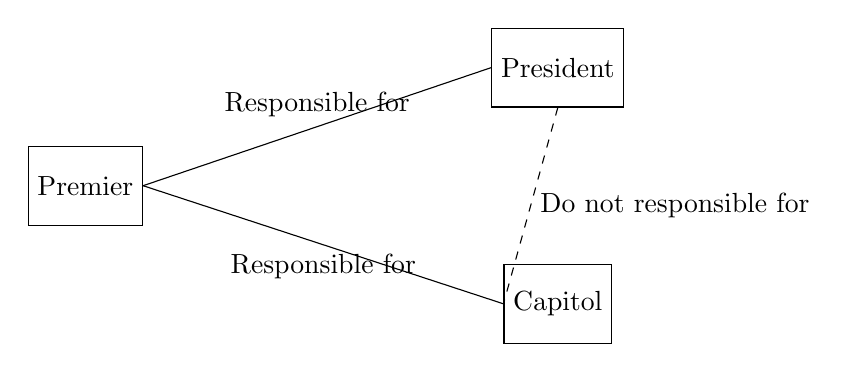
\begin{tikzpicture}
\node[draw, rectangle, minimum width=1cm, minimum height=1cm] (left) at (2, 0) {Premier};
\node[draw, rectangle, minimum width=1cm, minimum height=1cm] (topRight) at (8, 1.5) {President};
\node[draw, rectangle, minimum width=1cm, minimum height=1cm] (bottomRight) at (8, -1.5) {Capitol};
\draw[thin] (left.east) -- (topRight.west) node[midway, above] {Responsible for};
\draw[thin] (left.east) -- (bottomRight.west) node[midway, below] {Responsible for};
\draw[dashed] (topRight.south) -- (bottomRight.west) node[midway, right] {Do not responsible for};
\end{tikzpicture}
\end{center}
\begin{center}
Figure 1: An example of Semi-Presidential System.
\end{center}
\end{frame}
\begin{frame}{R.O.C. Semi-Presidential System}
  \begin{center}
  \begin{tikzpicture}
  \node[draw, rectangle, minimum width=1cm, minimum height=1cm] (bottomLeft) at (6, -1.5) {Judicial Yuan};
  \node[draw, rectangle, minimum width=1cm, minimum height=1cm] (topLeft) at (4, 1.5) {Supervisor Yuan};
  \node[draw, rectangle, minimum width=1cm, minimum height=1cm] (left) at (2, 0) {Examinator Yuan};
  \node[draw, rectangle, minimum width=1cm, minimum height=1cm] (topRight) at (10, 1.5) {Executive Yuan};
  \node[draw, circle, minimum size=0.3cm] (circleleft) at (2, -1.5) {銓敘部};
  \node[draw, rectangle, minimum width=1cm, minimum height=1cm] (bottomRight) at (9, -1.5) {Capitol};
  \draw[<->] (topRight.west) -- (bottomRight.north) node[midway, right] {Responsible for};
  \draw[->] (topLeft.south) -- (bottomRight.north) node[midway, right] {Supervisor to};
  \draw[->] (topLeft.east) -- (topRight.west) node[midway, below] {Supervisor to};
  \draw[->] (bottomLeft.north) -- (topRight.west) node[midway, above] {Check};
  \draw[->] (bottomLeft.east) -- (bottomRight.west) node[midway, above] {Check};
  \end{tikzpicture}
  \end{center}
\begin{center}
Figure 1: An example of R.O.C. Semi-Presidential System.
\end{center}
\end{frame}
\begin{frame}{}
\begin{center}
\Large{End of Chapter 1}
\end{center}
\end{frame}
\end{document}